\documentclass[%margin%,line,pifont,palatino,courier
]{article}
\usepackage{fullpage}
\usepackage{lastpage}
\usepackage[top=1in,bottom=1in,margin=1in]{geometry}
\usepackage{supertabular}
\usepackage{graphicx,tikz}	
%\usepackage{tkz-euclide}
%\usetkzobj{all}
%\usetikzlibrary{calc}
\usepackage{array,multicol}
\usepackage{amsmath,amssymb}
\usepackage{enumitem}

\usepackage{fancyhdr}
\pagestyle{fancy}

\addtolength{\topmargin}{-0.25in}

\newcommand{\vect}[1]{\mathbf{#1}}
\DeclareMathOperator{\proj}{proj}

\fancypagestyle{plain}{
	\addtolength{\headheight}{0.485in}
	\rhead{\bf MATH 235 (Calculus I) \\
		%\vspace{0.5pc}
		due Mon 16 Oct 2017 \\}
	\rfoot{\footnotesize THQuiz 4, p. \thepage\ (of \pageref{LastPage})
	}
\renewcommand{\headrulewidth}{0pt}
}
\fancyhf{}
\renewcommand{\headrulewidth}{0pt}
\rfoot{\footnotesize THQuiz 4, p. \thepage\ (of \pageref{LastPage})$\;$}

\title{\vspace{-3.5pc} 
	\flushleft \bf \Large Take-Home Quiz 4: Introduction to derivatives %\\ 
	 (\S2.1, 2.7-3.2)}
\date{}

% % % % %
\begin{document}
\maketitle

\vspace{-3pc}
\noindent{\bf Directions:} This quiz is due on October 16, 2017 at the beginning of lecture.  You may use whatever resources you like -- e.g., other textbooks, websites, collaboration with classmates -- to complete it \textbf{but YOU MUST DOCUMENT YOUR SOURCES}.  Acceptable documentation is enough information for me to find the source myself.  Rote copying another's work is unacceptable, regardless of whether you document it.  

\noindent\hrulefill

\begin{enumerate}
% % %
\item {\bf \S2.1 \#2} A cardiac monitor is used to measure the heart rate of a patient after surgery.  It copiles the number of heartbeats after $t$ minutes.  When the data in the table below are graphed, the slope of the tangent line represents the heart rate in beats per minute.
\begin{center}
\begin{tabular}{ r | l l l l l }
$t$ (min) & 36 & 38 & 40 & 42 & 44 \\
\hline
heartbeats & 2530 & 2661 & 2806 & 2948 & 3080
\end{tabular}
\end{center}
The monitor estimates this value by calculating the slope of a secant line.  	
	\begin{enumerate}
	\item Use the data to estimate the patient's heart rate after 42 minutes using the secant line between the points with the given values of $t$:
		\begin{itemize}
		\item $t=36$ and $t=42$
		\item $t=38$ and $t=42$
		\item $t=40$ and $t=42$
		\item $t=42$ and $t=44$
		\end{itemize}
	\item What are your conclusions?		
	\end{enumerate}

% % %
\item {\bf \S2.7 \#22} If the tangent line to $y=f(x)$ at $(4,3)$ passes through the point $(0,2)$, find $f(4)$ and $f'(4)$.
 
% % %
\item {\bf \S2.7 \#26} Sketch the graph of a function $f$ where 
	\begin{itemize}
	\item the domain is $(-2,2)$, 
	\item $f'(0)=-2)$, 
	\item $\lim_{x\to 2^-}f(x)=\infty$,
	\item $f$ is continuous at all numbers in its domain except $\pm 1$, and
	\item $f$ is odd.
	\end{itemize}

% % %
\item {\bf \S2.8 \#14} The graph (from the US Department of Energy) shows how driving speed affects gas mileage.  Fuel economy $F$ is measured in miles per gallon and speed $v$ is measured in miles per hour.
\begin{center}
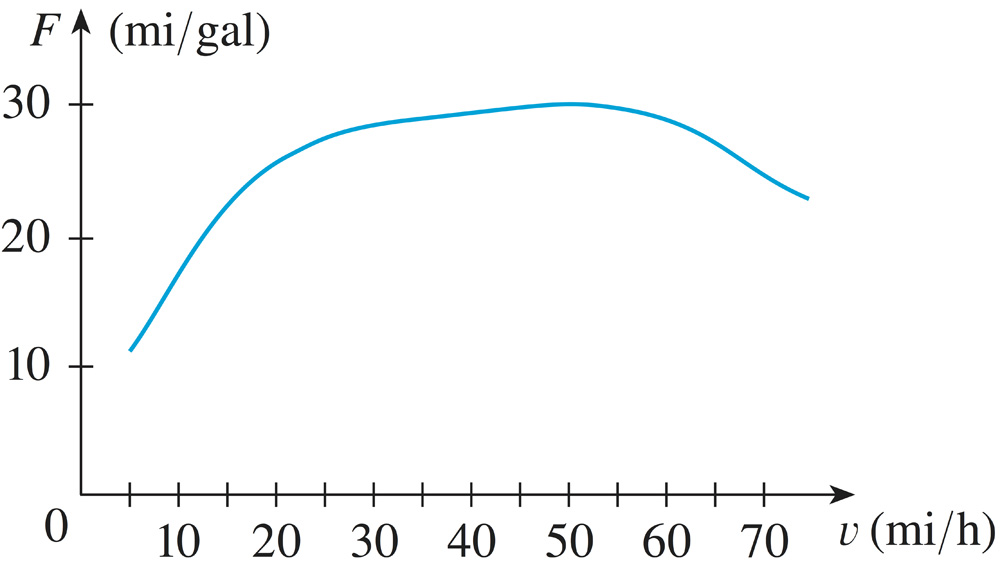
\includegraphics[scale=5]{2-8_12Stewart8Ed.jpg}
\end{center}
	\begin{enumerate}
	\item What is the meaning of the derivative $F'(v)$?
	\item Sketch the graph of $F'(v)$.
	\item At what speed should you drive if you want to save on gas?
	\end{enumerate}

\newpage
% % %
\item {\bf \S3.1 \#72} To show a function $f(x)$ is \textbf{differentiable} at a point $x=a$ you must show $\displaystyle\lim_{x\to a}\frac{f(x)-f(a)}{x-a}$ exists.  The following function $g$ is differentiable except for possibly at $x=0$ and $x=2$.
\[
g(x)=\begin{cases}
	2x & \text{ if } x\leq 0 \\
	2x-x^2 & \text{ if } 0<x<2 \\
	2-x & \text{ if } x\geq 2
	\end{cases}
\] 
	\begin{enumerate}
	\item Check the differentiability of $g$ at $x=0$ and $x=2$.  
	\item Give a formula for $g'$.
	\item Sketch the graphs of $g$ and $g'$ (on the same axes).
	\end{enumerate}

% % %
\item {\bf \S3.1 \#80} The general graph of the function $f(x)=ax^2+bx+c$ is a parabola.  Prove that the average of the slopes of the tangent lines to the parabola at the endpoints of any interval $[p,q]$ equals the slope of the tangent line at the midpoint of the interval.

% % %
\item {\bf \S3.2 \#56} Compute $Q'(0)$, where
\[
Q(x)=\frac{1+x+x^2+xe^x}{1-x-x^2-xe^x}.
\]
\textit{Hint: Write $\displaystyle Q(x)=\frac{f(x)}{g(x)}$.  Then use $f(0)$, $f'(0)$, $g(0)$, and $g'(0)$ to compute $Q'(0)$.}

% % % 
\item {\bf \S3.2 \#58} A manufacturer produces bolts of fabric with a fixed width.  The quantity $q$ of this fabric (measured in yards) that is sold is a function of the selling price $p$ (in dollars per yard), so we can write $q=f(p)$.  Then the total revenue earned with selling price $p$ is $R(p)=pf(p)$.
	\begin{enumerate}
	\item What does it mean, in the context of the problem, to say that $f(2)=10,000$ and $f'(2)=-350$?
	\item Assuming the values in part (a), find $R'(20)$ and interpret your answer.
	\end{enumerate}

	
% % % % %
\end{enumerate}
\end{document}